\chapter{Desenho do Projeto} 
\label{chap:Chapter06}

O objetivo central deste capítulo é descrever as decisões de design tomadas para o desenvolvimento da aplicação, com base nos requisitos funcionais e não funcionais identificados no capítulo anterior. Primeiramente, será apresentado o desenho da aplicação, onde serão detalhadas as funcionalidades e as estruturas da interface nos modos livre e desafio. Também serão descritos os recursos implementados para facilitar a navegação e a usabilidade, como feedbacks sonoros e teclas de atalho.

Em seguida, serão detalhadas as escolhas tecnológicas realizadas, como o uso do React e do TypeScript, fundamentando a escolha dessas tecnologias com base em suas características de leveza e facilidade no desenvolvimento. A escolha dessas tecnologias norteará as decisões arquiteturais e funcionais do projeto, garantindo uma experiência intuitiva e acessível aos usuários.

\section{Design da Interface}

O objetivo principal do projeto é oferecer uma aplicação com uma interface acessível e de fácil utilização, garantindo que qualquer pessoa, independentemente de sua condição visual, consiga usá-la sem dificuldades. Pensando nisso, a aplicação foi desenhada para que suas funcionalidades possam ser utilizadas tanto com o teclado quanto com o mouse, possibilitando que pessoas videntes, cegas ou com baixa visão possam interagir com a interface de forma independente e da maneira que preferirem. Essa abordagem, além de garantir a acessibilidade da aplicação, também contempla as principais necessidades dos usuários com deficiência visual.

A interface foi projetada para garantir um bom contraste visual, utilizando um fundo branco e texto preto. A escolha dessa combinação de cores visa atender pessoas com baixa visão, proporcionando boa legibilidade e uma experiência visual agradável para pessoas videntes que possam vir a utilizar a aplicação. Todos os botões e atalhos da aplicação são acompanhados de um feedback sonoro, permitindo que pessoas cegas ou aquelas que optem pela navegação por teclado tenham um retorno auditivo constante sobre suas ações.

\section{Estrutura do Menu Principal}

A aplicação apresenta um menu principal, onde são exibidos três botões principais: Modo Livre, Modo Desafio e Informações. No topo da interface, o nome da aplicação, 'Máquina Den Braille', é destacado, seguido dos botões de navegação. Todos esses elementos são acessíveis via mouse e teclado. Ao navegar pelos botões usando o teclado, o usuário pode alternar entre as opções com a tecla Tab e selecionar a função desejada com Enter. Cada troca de botão emite um som de confirmação, indicando em qual botão o usuário está focado, de modo a auxiliar na navegação.

Ao iniciar a aplicação, a primeira tela apresentada será o menu principal (figura \ref{fig:ch06-Menu principal}), onde são exibidos três botões: Modo Livre, Modo Desafio e Sobre, que dão acesso às suas respectivas interfaces. No topo da interface, o nome da aplicação, 'Máquina Den Braille', é destacado, seguido dos botões de navegação. A cada troca de botão, um som de confirmação é emitido para indicar em qual botão o usuário está focado, auxiliando assim sua navegação.

Quando a tela do menu principal é carregada, é emitido um áudio dizendo 'Menu principal da Máquina Den Braille'.

\begin{figure}[h]
    \centering
    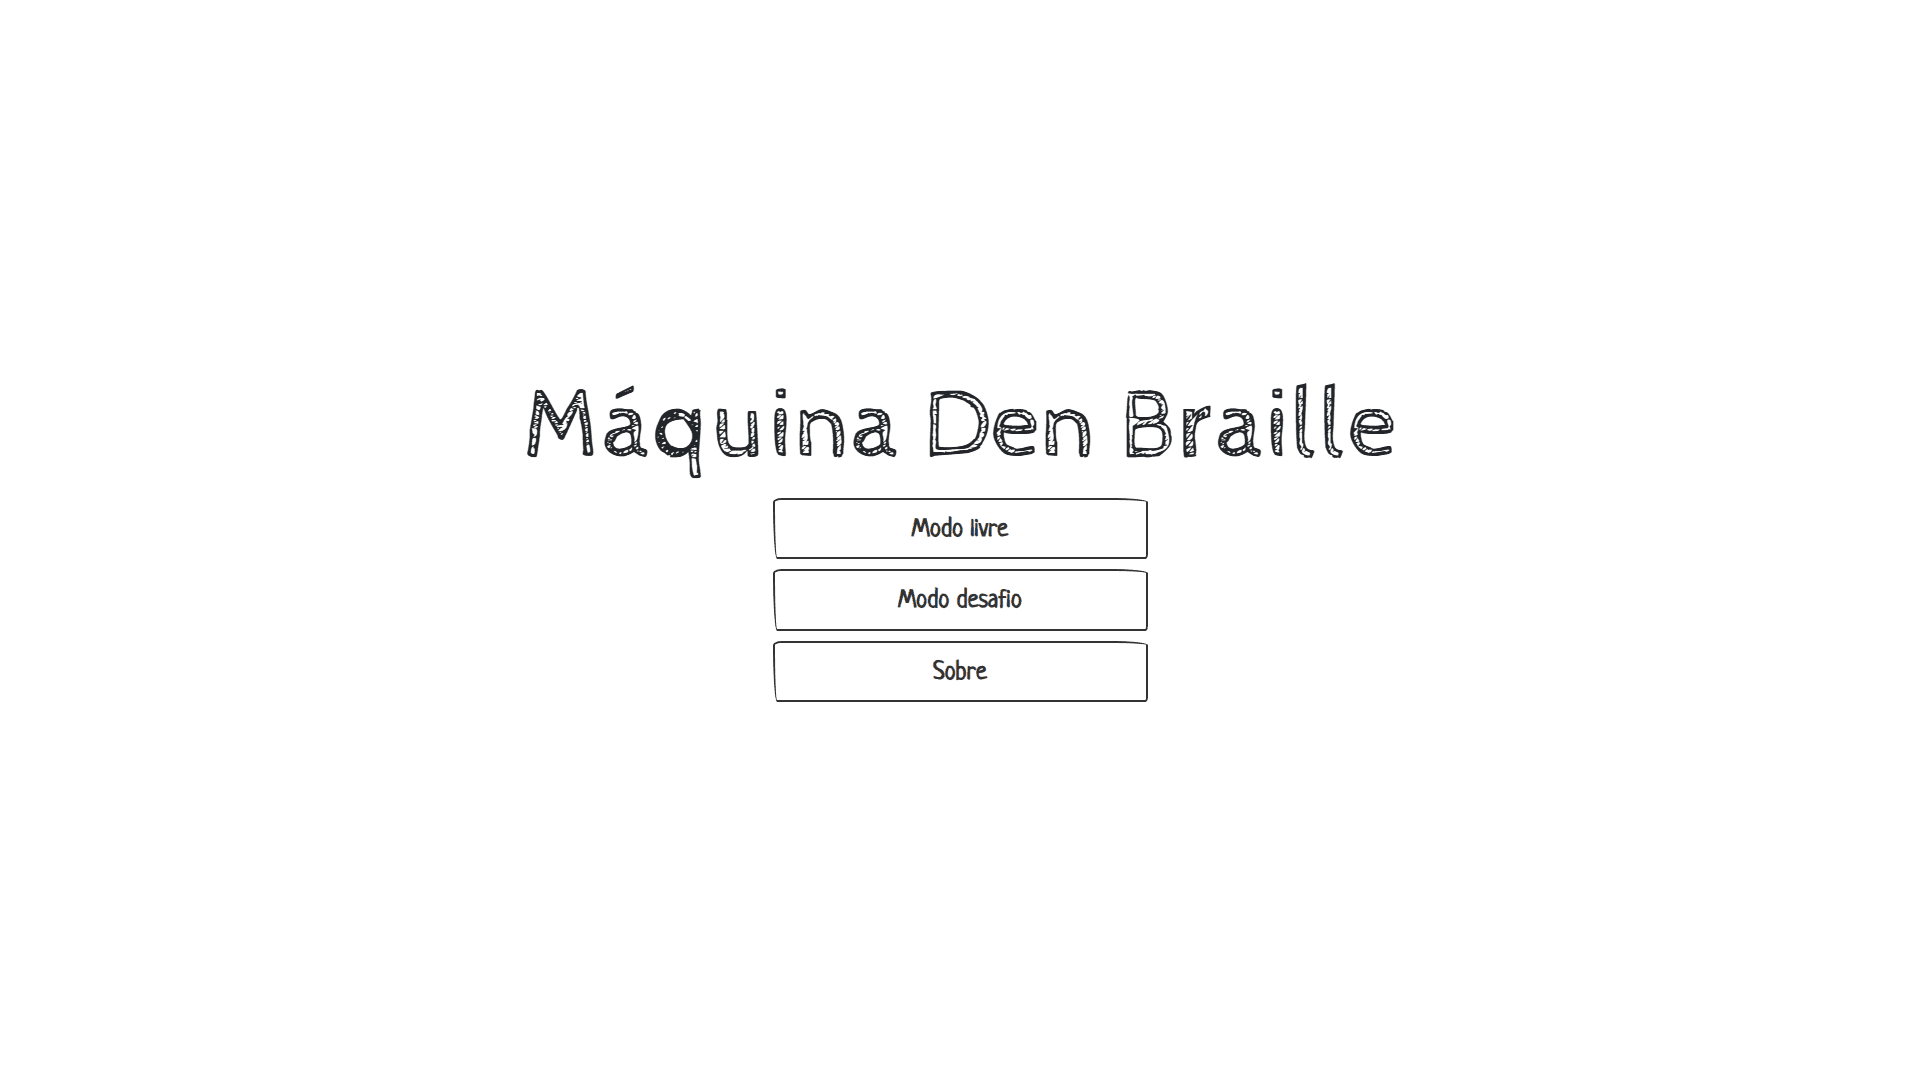
\includegraphics[scale=0.3]{ch06/assets/menu-principal.png}
    \decoRule
    \caption[Menu principal]{Menu principal da Máquina Den Braille}
    \label{fig:ch06-Menu principal}
\end{figure}

O nome 'Máquina Den Braille' é um trocadilho em homenagem à servidora do \gls{IFMA-MTC}, Denise Ferreira Costa, que foi a pessoa que me apresentou ao mundo das pessoas com deficiência visual, sendo ela quem me ensinou braille. A palavra esperada 'de' é substituída por 'Den', fazendo referência ao início do nome 'Denise'.

\section{Funcionamento do Modo Livre}

O objetivo do modo livre é proporcionar ao usuário um ambiente para praticar livremente a escrita em braille, simulando a experiência de escrita em uma máquina de escrever em braille física. Ao acessar a tela do modo livre (figura \ref{fig:ch06-Modo Livre}), o usuário ouvirá a mensagem de introdução: 'Pressione 'i' para ouvir as instruções'. Essa mensagem serve para orientar os usuários quanto ao acesso opcional às instruções de uso do simulador, evitando a repetição desnecessária para aqueles que já estão familiarizados com os comandos básicos da aplicação.

Quando o usuário pressionar a tecla 'i', ele ouvirá um áudio com instruções detalhadas sobre a utilização do simulador. Esse áudio contém orientações sobre quais teclas do teclado representam os pontos da cela braille na máquina real, além do uso das teclas de espaço, apagar e quebra de linha. O áudio também inclui instruções sobre os atalhos de acessibilidade, como a visualização do texto a tinta, ativação e desativação do som da conversão para braille e o som das teclas pressionadas. Essas instruções foram incluídas para assegurar que a experiência do usuário seja intuitiva e inclusiva, com todas as funcionalidades claramente descritas em áudio.

\begin{figure}[h]
    \centering
    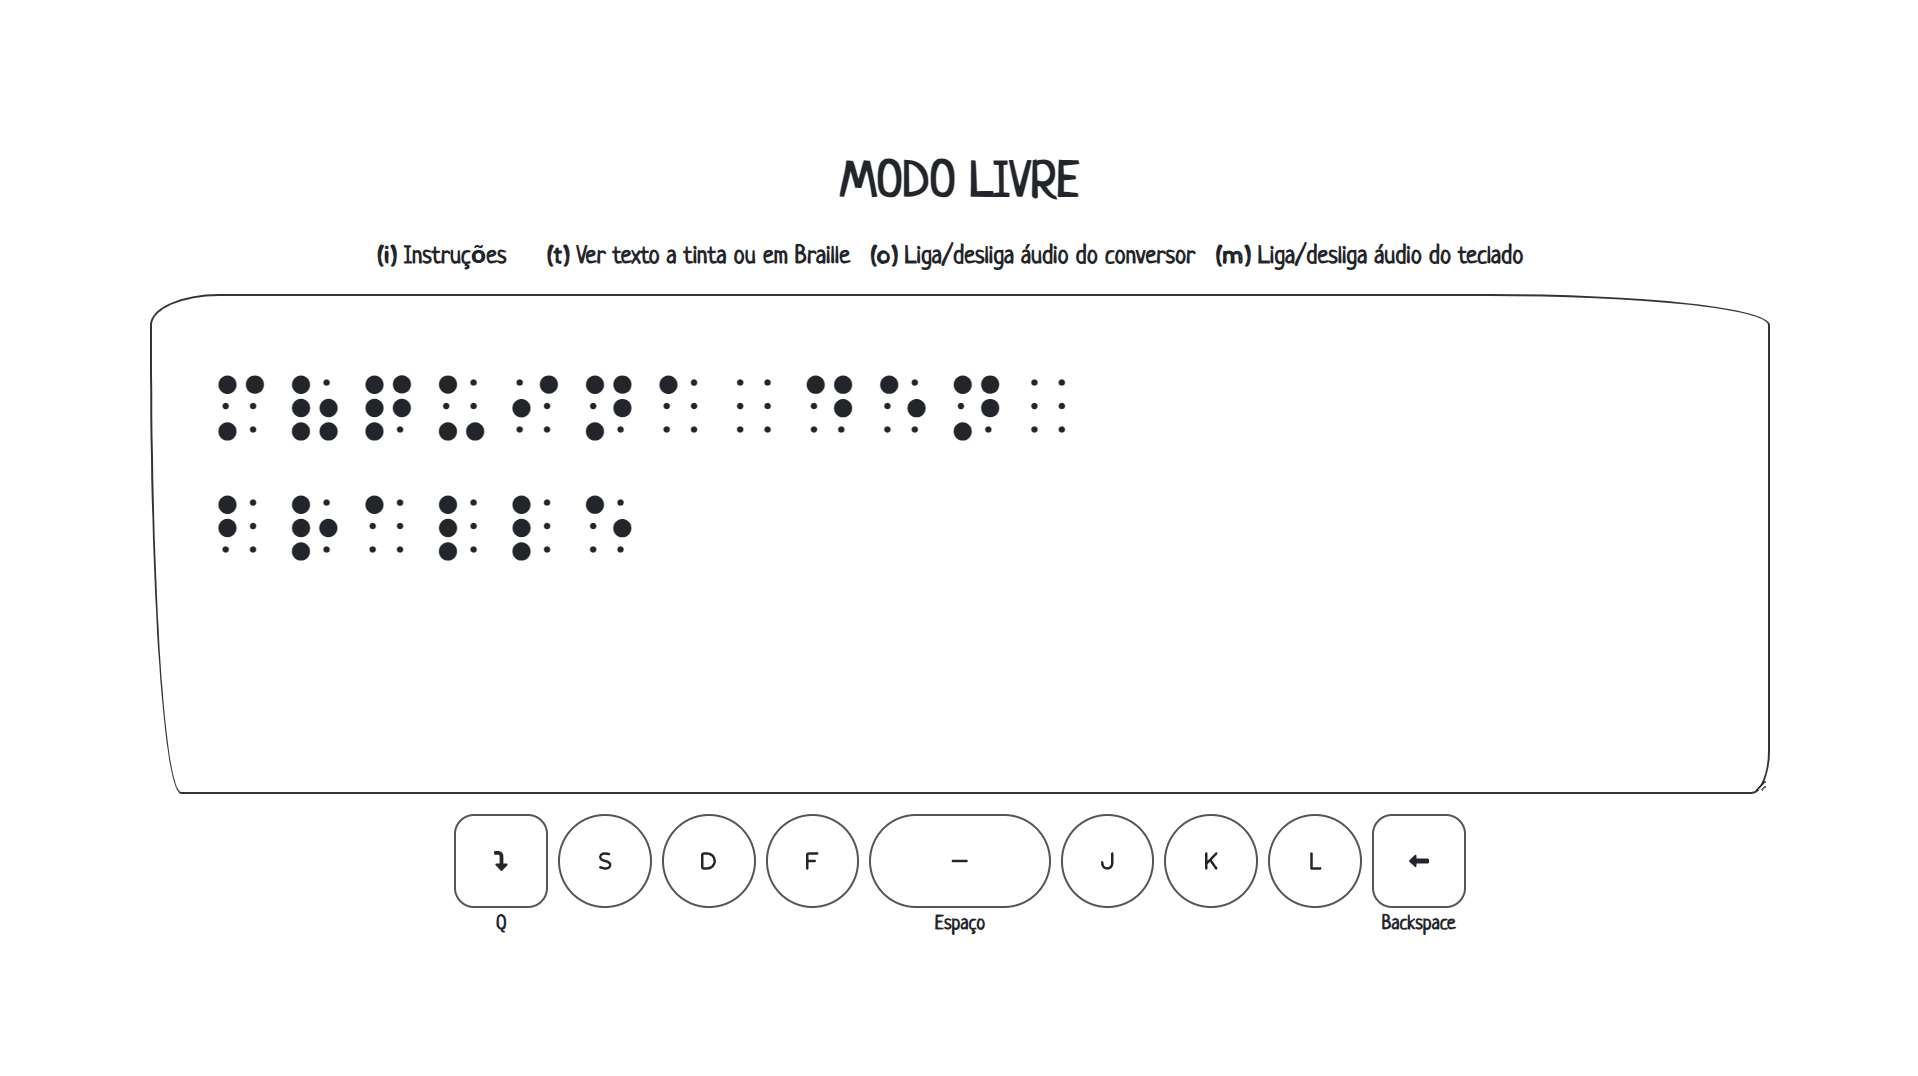
\includegraphics[scale=0.3]{ch06/assets/modo-livre.png}
    \decoRule
    \caption[Modo Livre]{Modo Livre da Máquina Den Braille}
    \label{fig:ch06-Modo Livre}
\end{figure}

Como mostra a figura \ref{fig:ch06-Modo Livre}, o layout da interface do modo livre foi planejado para lembrar a aparência da máquina física. Um título indicativo, 'Modo Livre', está localizado na parte superior da tela, seguido por uma seção informativa que lista os atalhos mais importantes, já explicados no áudio de instruções. 

Logo abaixo, há a área de exibição do 'papel', onde o texto digitado pelo usuário é apresentado, primeiramente em braille, com a possibilidade de alternar para a visualização do texto a tinta por meio da tecla de atalho 't'.

Para a apresentação do texto em Braille na aplicação, foi utilizada uma versão modificada da fonte 'Borthick's Braille', criada por Steven Borthick em 2006 e disponibilizada no site \url{dafont.com}. O design original da fonte foi preservado, e as adaptações realizadas visaram a adequação da fonte à grafia Braille para português, como mostra o exemplo na figura \ref{fig:ch06-Editor da Fonte Braille}. As modificações incluíram a adição de caracteres Braille ausentes na versão original e o remapeamento dos sinais para corresponderem à grafia Braille utilizada em português. Essas adaptações foram implementadas utilizando a plataforma \url{tophix.com}, que permite tanto a modificação do design quanto o mapeamento dos caracteres para símbolos específicos.

\begin{figure}[h]
    \centering
    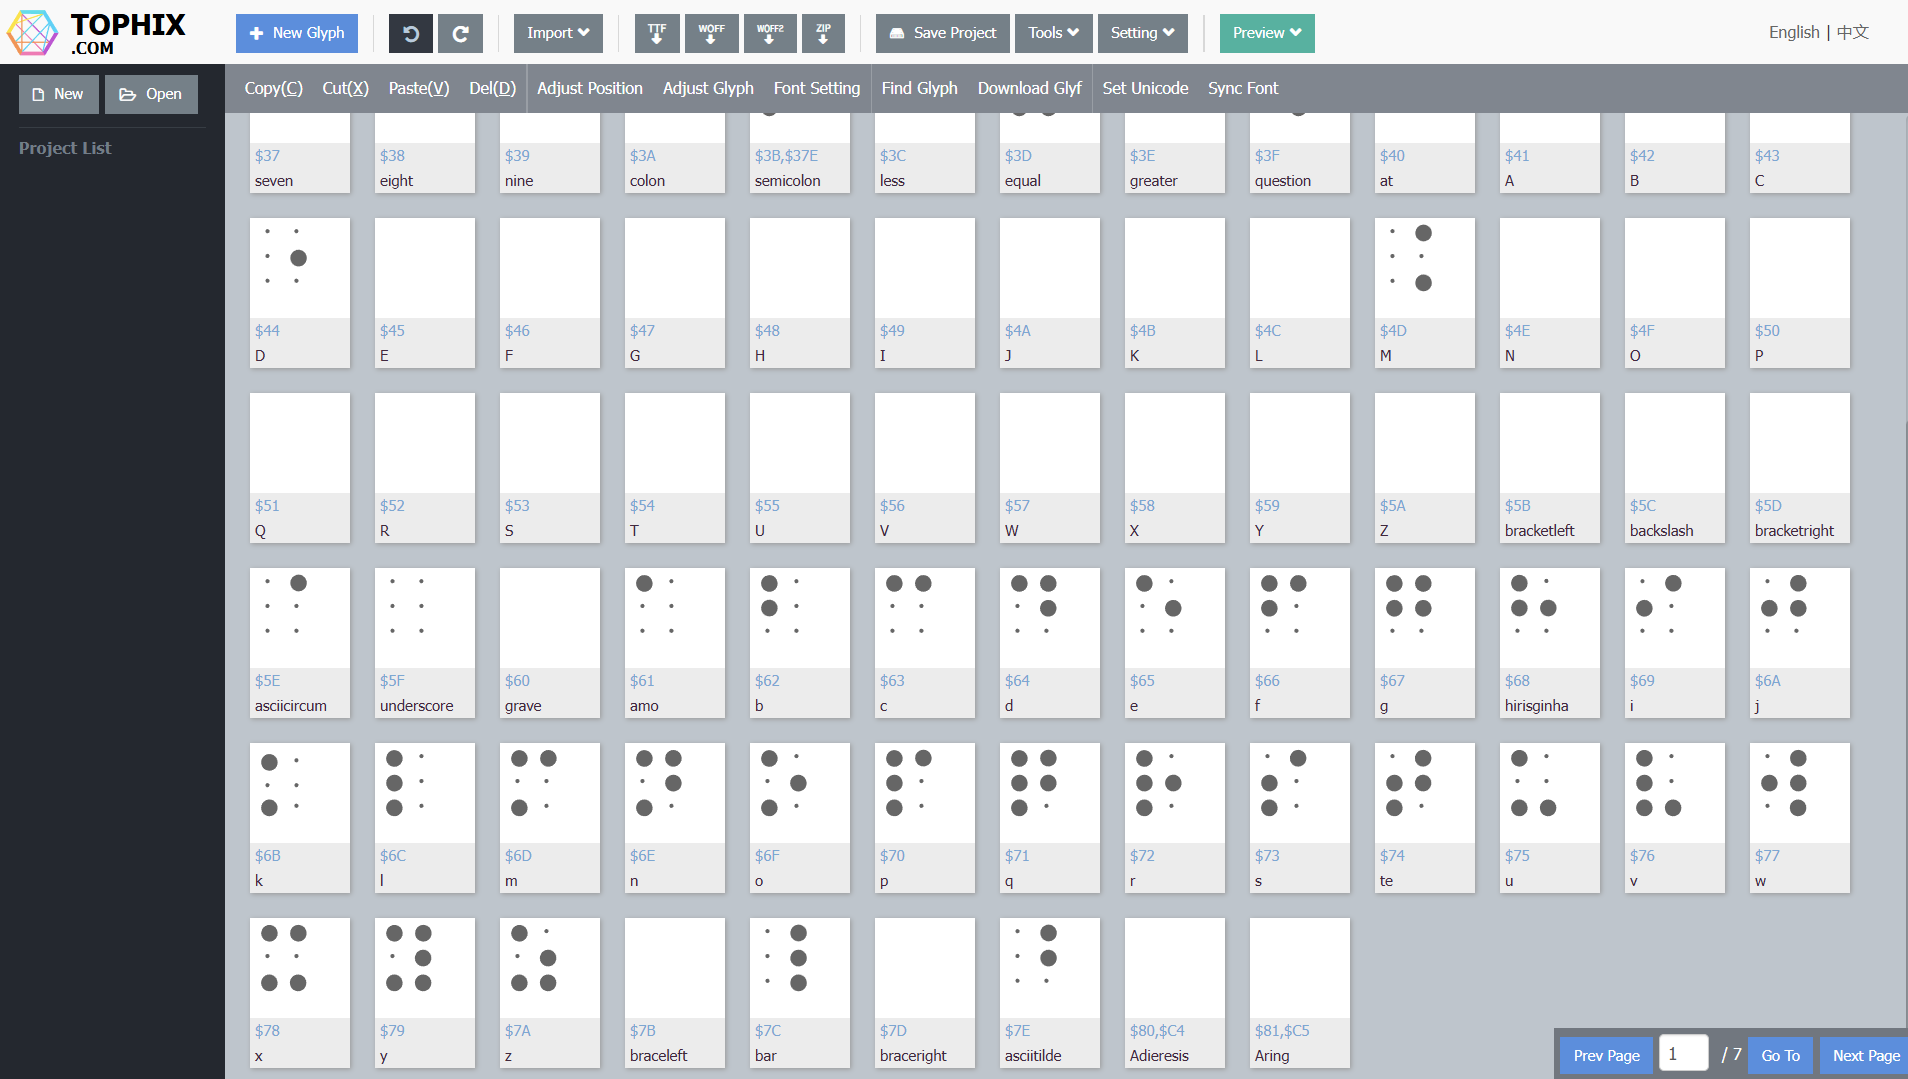
\includegraphics[scale=0.3]{ch06/assets/editor-fonte.png}
    \decoRule
    \caption[Editor da Fonte Braille]{Editor da Fonte Braille}
    \label{fig:ch06-Editor da Fonte Braille}
\end{figure}

Para garantir que o usuário pudesse diferenciar com clareza os pontos ativos e inativos em cada célula Braille, foram adotados dois tamanhos distintos de círculos, como mostra a figura \ref{fig:ch06-fonte-braille}: um círculo de maior diâmetro para representar os pontos ativados (em relevo) e um círculo menor para os pontos não utilizados naquela combinação.

\begin{figure}[h]
    \centering
    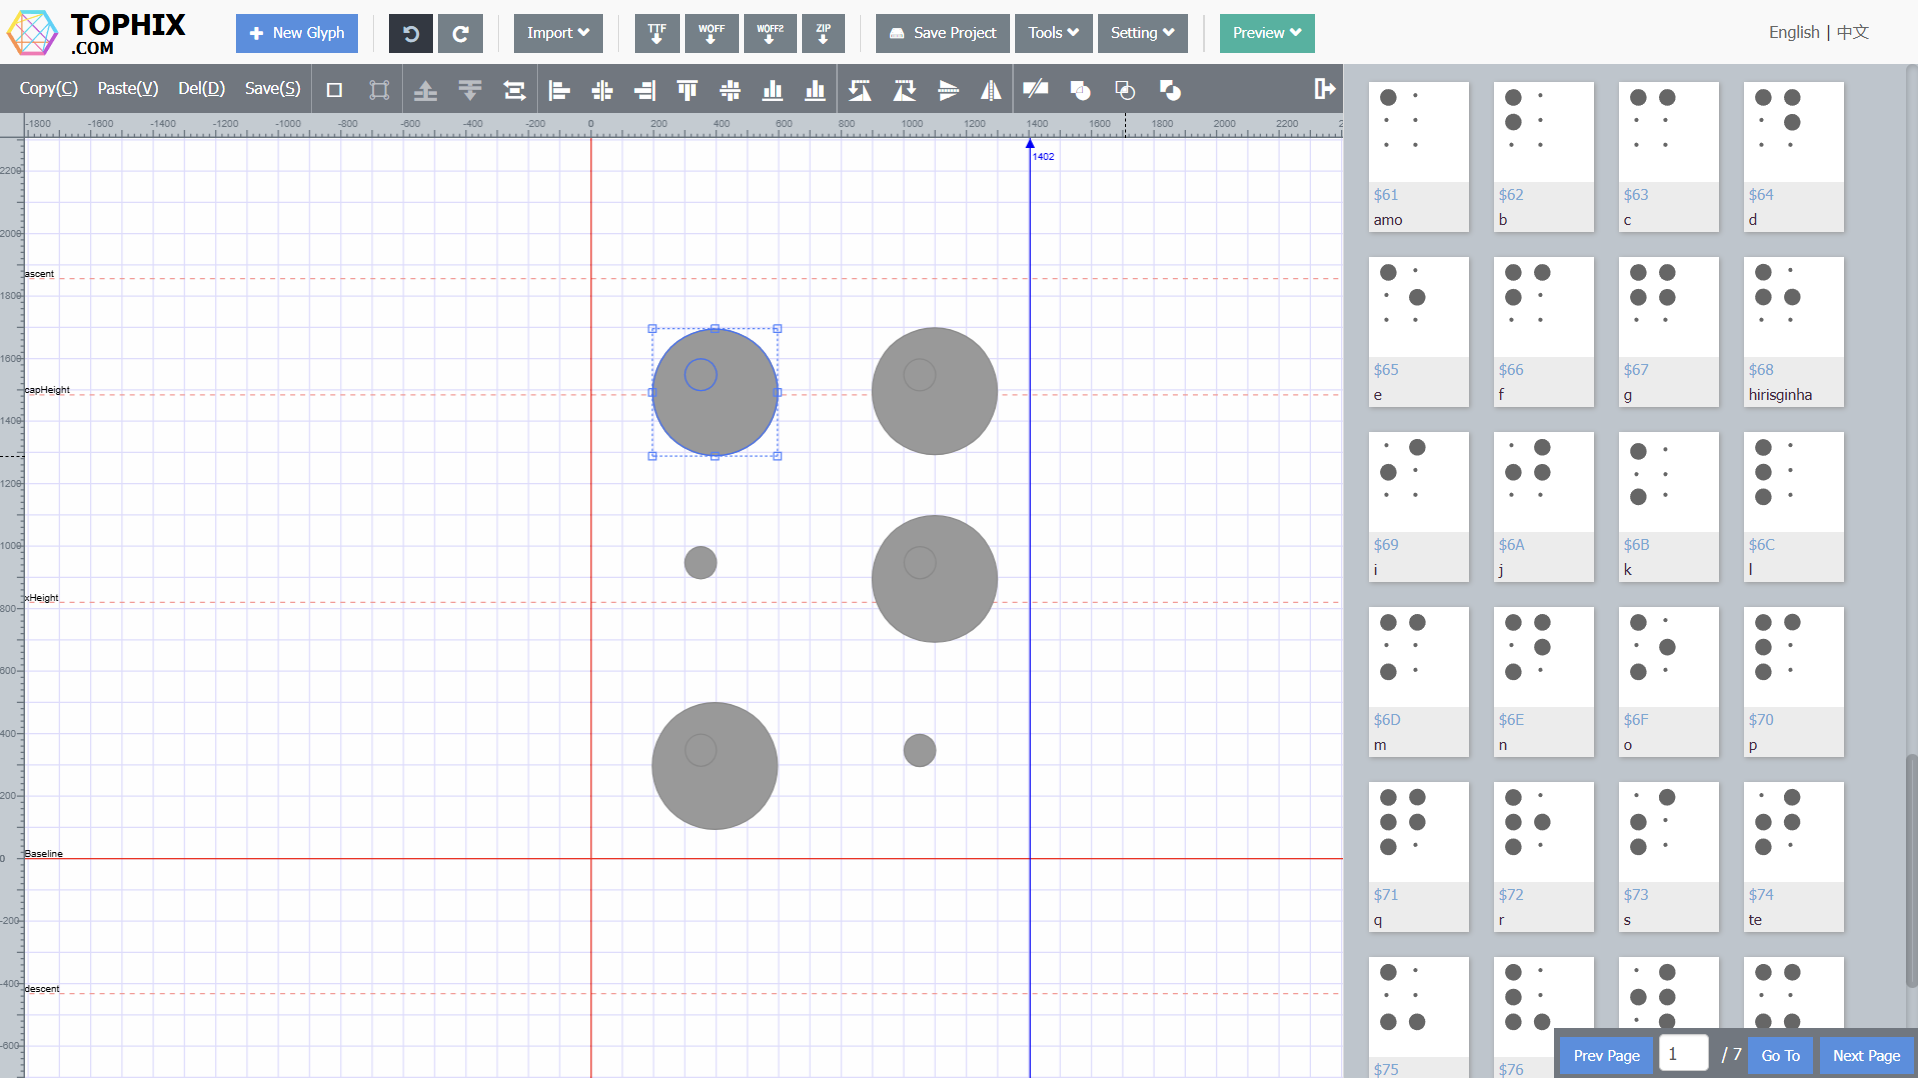
\includegraphics[scale=0.3]{ch06/assets/font-braille.png}
    \decoRule
    \caption[Fonte Braille]{Fonte Braille}
    \label{fig:ch06-fonte-braille}
\end{figure}

Abaixo da área de exibição, estão representadas as teclas da máquina braille. Algumas teclas são representadas por círculos, outras por quadrados ou retângulos com cantos arredondados, e cada tecla possui uma função específica, como é visto na figura \ref{fig:ch06-Teclas do Simulador}. 

\begin{figure}[h]
    \centering
    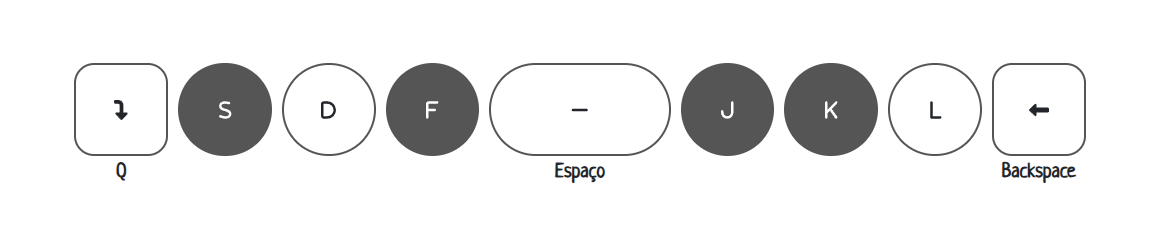
\includegraphics[scale=0.5]{ch06/assets/teclas-do-simulador.png}
    \decoRule
    \caption[Teclas do Simulador]{Teclas do Simulador}
    \label{fig:ch06-Teclas do Simulador}
\end{figure}

A tecla 'Q' é usada para quebras de linha. Sua visualização é em um quadrado com cantos arredondados e uma seta apontando para baixo, indicando que, ao pressioná-la, o usuário passará a digitar na linha abaixo. Abaixo da tecla, há a letra 'q' para lembrar ao usuário que é a tecla 'q' do teclado que ativa essa função. 

As teclas 'S', 'D' e 'F' correspondem aos pontos '3', '2' e '1' da cela braille e são representadas por círculos contendo a letra correspondente no teclado. 

A tecla de espaço é representada por um retângulo com cantos arredondados, contendo apenas um traço e, abaixo, a palavra 'espaço', para lembrar ao usuário que a tecla de espaço do teclado faz a função de uma cela vazia na máquina braille. 

As teclas 'J', 'K' e 'L' representam os pontos '4', '5' e '6' da cela braille e também são representadas por círculos, contendo sua respectiva letra correspondente. 

Por fim, a tecla 'Backspace' é usada para apagar uma cela. Na interface, é representada por um quadrado com cantos arredondados, contendo uma seta para a esquerda e, abaixo, a palavra 'backspace'. Essa última tecla foi implementada de forma adaptativa, uma vez que as máquinas braille físicas não oferecem a funcionalidade de apagar pontos diretamente. Esse recurso foi incluído para facilitar o uso, permitindo que o usuário corrija erros sem a necessidade de recomeçar o que estava escrevendo.

Ao pressionar uma ou mais teclas de pontos simultaneamente, a aplicação irá gerar uma cela braille correspondente na área do papel. Imediatamente após isso, o conversor de braille para texto a tinta reproduzirá um som informando o caractere gerado. Caso a tecla pressionada não seja uma tecla de ponto, o simulador executará a ação correspondente, e o conversor reproduzirá um som indicando qual ação foi executada. A parte sonora contribui para o aprendizado do usuário e reforça a confirmação de suas ações.

\section{Funcionamento do Modo Desafio}

O modo desafio oferece uma prática mais interativa, propondo ao usuário desafios de digitação de palavras em braille. Ao acessar a tela do modo desafio, o usuário ouvirá novamente a mensagem "Pressione 'i' para ouvir as instruções". Nessa interface, as instruções detalham como utilizar o simulador no modo desafio, assumindo que o usuário já conhece as funções básicas da aplicação.

A interface do modo desafio é ligeiramente diferente da interface do modo livre, como pode ser observado na figura \ref{fig:ch06-Modo Desafio}. Suas diferenças incluem o título, que agora exibe "Modo Desafio", a palavra atual do desafio logo abaixo do título, e algumas instruções adicionais sobre teclas de atalho. As novas teclas utilizadas no modo desafio são 'r', para ouvir a palavra atual, e 'Enter', para confirmar a resposta. Quando a tela do modo desafio é carregada, uma palavra já é selecionada aleatoriamente a partir da base de palavras da aplicação.

\begin{figure}[h]
    \centering
    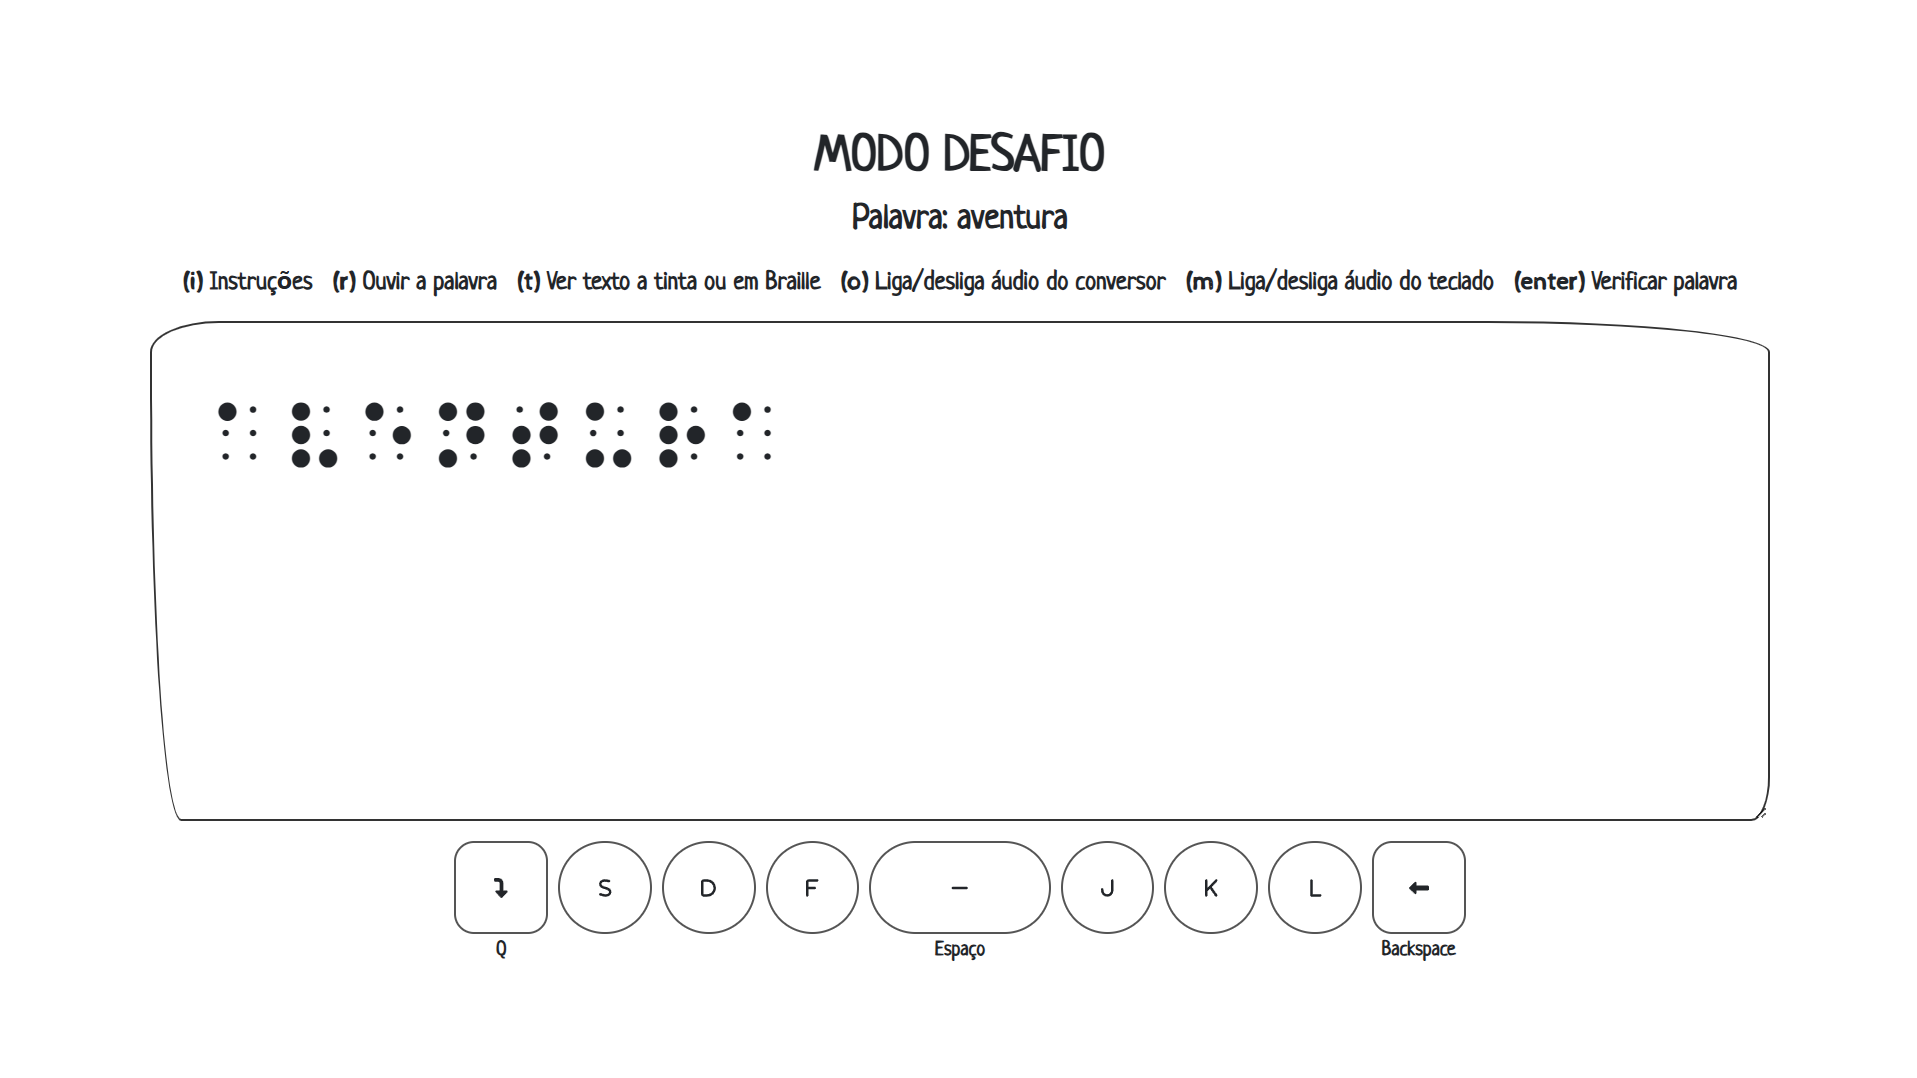
\includegraphics[scale=0.3]{ch06/assets/modo-desafio.png}
    \decoRule
    \caption[Modo Desafio]{Modo Desafio da Máquina Den Braille}
    \label{fig:ch06-Modo Desafio}
\end{figure}

O usuário ouvirá uma palavra que deve ser escrita em braille utilizando o simulador. A cada desafio, uma nova palavra é escolhida aleatoriamente entre uma lista de palavras existentes na aplicação, abrangendo todas as letras do alfabeto português, incluindo alguns caracteres acentuados. O objetivo é que o usuário digite em braille a palavra ouvida e, ao final, pressione 'Enter' para verificar se sua resposta está correta. Em caso de erro, o usuário poderá tentar novamente, recebendo um novo feedback auditivo para saber se sua resposta está correta ou não. Esse formato de desafio reforça o aprendizado ao exigir maior precisão e atenção do usuário no momento da escrita em braille.

\section{Tecnologias Utilizadas}

Para atender ao objetivo central de simplicidade e acessibilidade, o simulador foi desenvolvido como uma aplicação web leve e de fácil acesso, eliminando a necessidade de instalação de software ou de um hardware potente. A aplicação pode ser acessada diretamente pelo navegador, bastando ao usuário ter um dispositivo com conexão à internet. As tecnologias selecionadas para a construção deste projeto foram React.js, TypeScript, HTML e CSS.

\subsection{HTML e CSS}

HTML (HyperText Markup Language) é a linguagem de marcação padrão utilizada para estruturar e exibir conteúdos na web \parencite{SITE01}. No desenvolvimento de interfaces web, o HTML fornece toda a estrutura necessária para organizar os elementos de uma página. É com o HTML que definimos a estrutura de botões, menus, disposição de textos, imagens, etc. Sendo a linguagem base de qualquer aplicação web, o HTML é indispensável para a organização da estrutura visual e funcional da interface.

CSS (Cascading Style Sheets) é a linguagem de estilo utilizada para personalizar a aparência e o layout de páginas HTML. Com o CSS, definimos cores, tamanhos, espaçamentos e outras características de estilo nas nossas páginas, dando estética e usabilidade à aplicação \parencite{SITE02}.

No contexto desta aplicação, grande parte da estilização foi feita utilizando a biblioteca de CSS chamada Bootstrap \parencite{SITE05}, especificamente uma versão modificada disponível no site Bootstrap Watch \parencite{SITE06}, chamada Bootstrap Sketchy, que permitiu que a interface tivesse uma aparência de "desenho à mão". 

\begin{figure}[h]
    \centering
    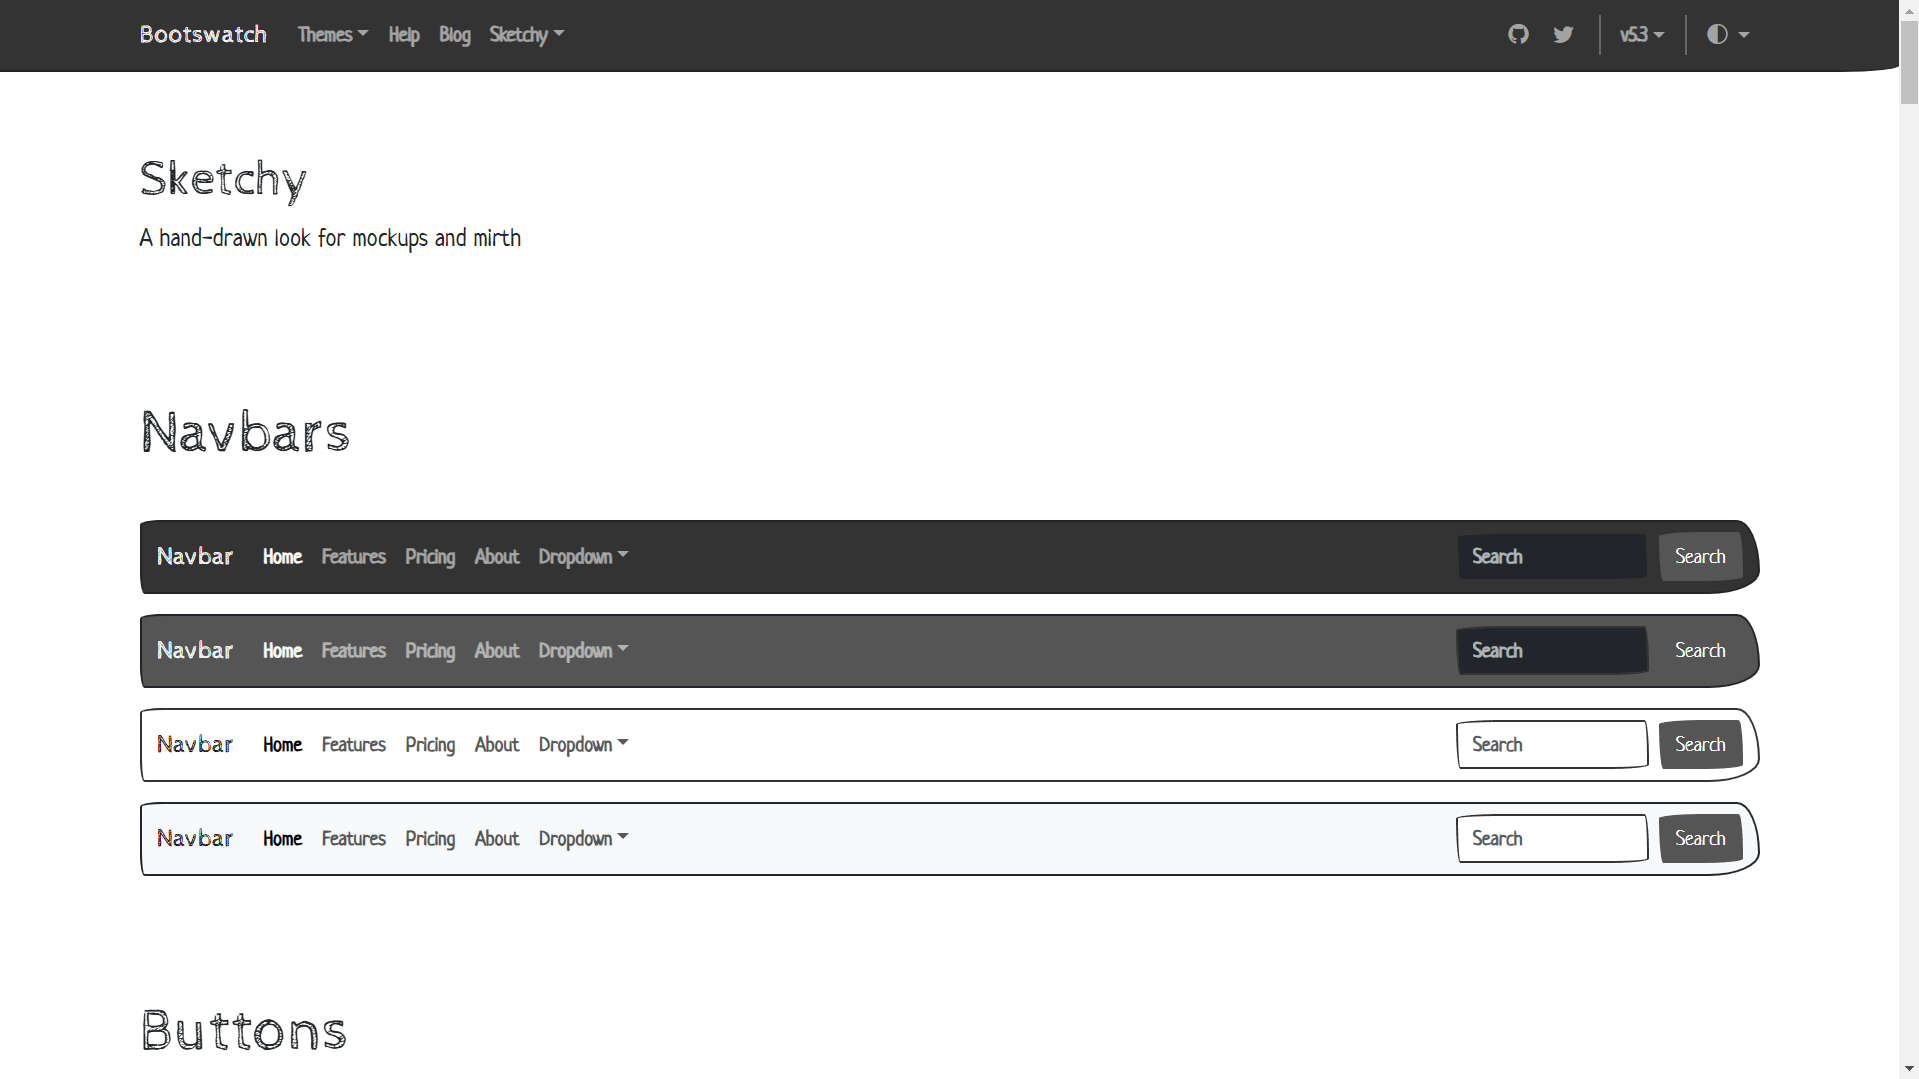
\includegraphics[scale=0.25]{ch06/assets/bootstrap-sketchy.png}
    \decoRule
    \caption[Bootstrap Sketchy]{Versão modificada do Bootstrap, chamada Bootstrap Sketchy}
\end{figure}

A escolha desse estilo foi feita para que a interface não tivesse uma aparência tão monótona, proporcionando uma experiência visual mais agradável para pessoas videntes ou com baixa visão.

\subsection{React}

O React é uma biblioteca JavaScript de código aberto, desenvolvida pela equipe do Facebook, amplamente utilizada para o desenvolvimento de interfaces de usuário, especialmente em aplicações de página única (Single Page Applications - SPAs) \parencite{SITE03}. O React possibilita a modularização do projeto, permitindo ao desenvolvedor criar componentes reutilizáveis, o que facilita a manutenção e a escalabilidade do código. No React, cada componente pode representar uma parte isolada da interface e ser atualizado de forma independente. Isso permite que sistemas desenvolvidos em React sejam rápidos, reativos e dinâmicos.

A escolha do React foi baseada em sua eficiência no gerenciamento de componentes e na sua arquitetura baseada em um Virtual DOM, que melhora o desempenho da aplicação ao reduzir a necessidade de renderizações completas, visto que a aplicação estará constantemente atualizando sua visualização.

\subsection{TypeScript}

TypeScript é uma linguagem de programação de código aberto desenvolvida pela Microsoft, que adiciona tipagem estática ao JavaScript. Isso significa que os tipos de variáveis, parâmetros e retornos de função são definidos de forma explícita, o que contribui para maior segurança e previsibilidade no código, ajudando a identificar erros em tempo de compilação \parencite{SITE04}. TypeScript é frequentemente utilizado em conjunto com React, pois traz maior robustez ao código, reduzindo a probabilidade de erros, especialmente em aplicações de larga escala \parencite{SITE03}.

A escolha do TypeScript neste projeto visa assegurar uma estruturação mais rigorosa do código, permitindo uma melhor organização da lógica que transforma os comandos do teclado em células braille e garantindo que o comportamento da aplicação seja consistente e previsível, aumentando a confiabilidade do código.


